\documentclass[12pt,a4paper]{scrartcl}

%%%%%
% Header for solutions for the course Machine Learning for Computer Vision
% Summer 2017
%%%%%

\usepackage[utf8]{inputenc}
\usepackage[english]{babel}

\usepackage{
  amsmath,
  graphicx,
  tabularx,
  caption,
  subcaption,
  float,
  listingsutf8,
}

\usepackage[load-configurations = abbreviations]{siunitx}
\usepackage{hyperref}
\usepackage[english]{cleveref}

%%%%% format settings
%------------
% \setlength{\parindent}{0pt} %no indent
%------------

%%%%% settings for listings
\lstset{
  language=python,
  basicstyle=\footnotesize,  % font size
  showspaces=false,
  showstringspaces=false,
  frame=single, %tb
  breaklines=true,
  % backgroundcolor=\color[RGB]{245,245,244},
  % otherkeywords={self},             % Add keywords here
  % keywordstyle=\color{blue},
  % commentstyle=\it\color[RGB]{0,96,96}\ttfamily,
  % stringstyle=\color[RGB]{255,140,0},
  % numbers=left,
  % stepnumber=5,
}

%%% commands
%------------
\newcommand{\code}{\texttt}
%------------


\author{Kodai Matsuoka, Yuyan Li}
\subject{Machine Learning for Computer Vision}
\title{Exercise 12}
% \subtitle{}
\date{24.07.2017}


\begin{document}

\maketitle

\section{Results}

\subsection{Distribution of rewards}
Change of distribution of reward and threshold is shown in figure 1 and 2.

\begin{figure}
	\centering
	\caption{Change of distribution of reward, 300 n\_samples, 50 percentile}
   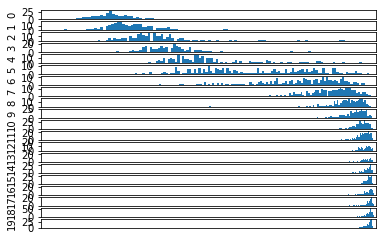
\includegraphics[width=15cm]{result1.png}
\end{figure}


\begin{figure}
	\centering
	\caption{Chanege of threshold, 300 n\_samples, 50 percentile}
    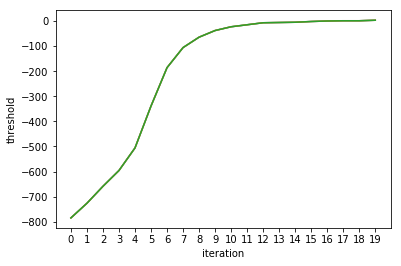
\includegraphics[width=15cm]{result2.png}
\end{figure}

As iterations are repeated, the distribution moves towards positive direction. The distribution makes no more improve after 15 iteration.

\subsection{How the algorithm performance changes if we change n\_samples and percentile}
We used 200, 500 and 1000 n\_samples. For each case, we changed percentile from 10\% to 90\% . The result is shown in Figure3.
When n\_samples = 200, mean reward was never above 0. If number of samples are enough many (500, 1000), we got satisfying result most of the time. However percetile should be chosen between 20\% and 80\%.


\begin{figure}
	\centering
	\caption{The relation between percentile and mean reward with defferent n\_samples}
    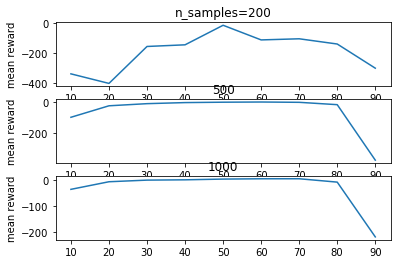
\includegraphics[width=15cm]{result3.png}
\end{figure}

\subsection{Tune the algorithm \& Bonus}
We achieved both positive mean reward and 25\% of samples above +9.0 with 1000 n\_samples using 50\% samples for learning. In this setting, the mean reward was +3.9, and 28\% of samples were above +9.0.


% \lstinputlisting[language=LANG,caption=CAPTION,label=lst:LABEL]{PATH/TO/CODE.file}

\section{Code}
\lstinputlisting[linerange={1-72}]{exercise12.py}

\end{document}